% !TeX program = pdflatex
\documentclass[tikz,border=8pt]{standalone}
\usepackage{pgfplots}\pgfplotsset{compat=1.16}
\definecolor{FigureBlue}{HTML}{2563EB}\definecolor{FigureOrange}{HTML}{EA580C}
\begin{document}
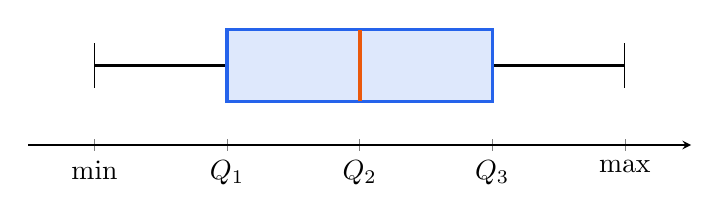
\begin{tikzpicture}
\begin{axis}[width=10cm,height=3.6cm,axis y line=none,axis x line=middle,xmin=0,xmax=10,ymin=0,ymax=2,xtick={1,3,5,7,9},xticklabels={min,$Q_1$,$Q_2$,$Q_3$,max},ytick=\empty,clip=false]
  \addplot[only marks,mark=|,mark size=8pt] coordinates {(1,1)(9,1)};
  \draw[line width=1.1pt] (axis cs:1,1)--(axis cs:3,1) (axis cs:7,1)--(axis cs:9,1);
  \draw[FigureBlue,fill=FigureBlue!15,line width=1.2pt] (axis cs:3,.55) rectangle (axis cs:7,1.45);
  \draw[FigureOrange,line width=1.5pt] (axis cs:5,.55)--(axis cs:5,1.45);
\end{axis}
\end{tikzpicture}
\end{document}
